\documentclass[draft,article]{UsydReport}

%% Variable Definitions %%
\newcommand{\reporttitle}{AERO2705 - Space Engineering 1 \\[1Em] Assignment Style Guide}
\newcommand{\authorname}{Prepared by: Julian Guinane}
\newcommand{\authorSID}{}

\title{Title}
\author{Author}
\date{\today}

\begin{document}
\frontmatter
\begin{titlepage}

\newcommand{\HRule}{\rule{\linewidth}{0.5mm}}
% Defines a new command for the horizontal lines, change thickness here

\center % Center everything on the page
 
%----------------------------------------------------------------------------------------
%	HEADING SECTIONS
%----------------------------------------------------------------------------------------

\textsc{\LARGE University of Sydney}\\[1.5cm] % Name of your university/college


%----------------------------------------------------------------------------------------
%	TITLE SECTION
%----------------------------------------------------------------------------------------

\HRule \\[0.4cm]
{ \huge \bfseries \reporttitle}\\[0.4cm] % Title of your document
\HRule \\[1.5cm]
 
%----------------------------------------------------------------------------------------
%	AUTHOR SECTION
%----------------------------------------------------------------------------------------

\begin{minipage}{0.4\textwidth}
\begin{center}\large 
\authorname\\\vspace{1cm}
Access the \href{https://github.com/Julian-Guinane/AERO2705-Report-Template}{GitHub Repo here}.
\authorSID\\\vspace{1cm}


% ADD YOUR SID
\end{center}
\end{minipage}
\vspace{1mm}

% If you don't want a supervisor, uncomment the two lines below and remove the section above
%\Large \emph{Author:}\\
%John \textsc{Smith}\\[3cm] % Your name

%----------------------------------------------------------------------------------------
%	DATE SECTION
%----------------------------------------------------------------------------------------

{\large \today}\\[2cm] % Date, change the \today to a set date if you want to be precise

%----------------------------------------------------------------------------------------
%	LOGO SECTION
%----------------------------------------------------------------------------------------


\includegraphics[width=0.5\textwidth]{Images/USYDlogo.jpg} % Include a department/university logo - this will require the graphicx package
 
%----------------------------------------------------------------------------------------

\vfill % Fill the rest of the page with whitespace
\end{titlepage}
% \maketitle
\newpage
\tableofcontents
% \newpage
% \listoffigures
% \newpage
% \listoftables

\newpage
\mainmatter
\section{Overview}
This is a brief style guide that you can refer to when completing your your AERO2705 assignments. While other subjects may have modified style rules, this should be a handy reference for completing reports generally. This is by no means an exhaustive list, so always use your common sense when formatting your assessments and ask questions if you are unsure.

\section{Report Structure}
When writing up an assignment, always clearly structure your report with numbered headings and subheadings. Some reports use a standard format sectioned as Introduction, Methodology,  Results and Discussion, and Conclusions. In some cases, it might be better to structure your report with respect to assignment questions (i.e. sectioned as Question 1, Question 2, Question 3). In longer or more formal reports, it is best to include a title page and table of contents, as is shown in this document. These pages are generally not included in page counts, and as such are numbered using roman numerals. Otherwise, a title heading on the first page is sufficient. Remember never to include your name on assessments. Always use your SID.

Where a page format and font size is not specified, assume standard 1-inch margins and use a font size of at least 11 pt. Remember also that concise, grammatically correct writing is very important. Alongside normal spellcheckers, \href{https://app.grammarly.com/}{Grammarly} is a great tool to help you improve your writing.

\section{Equations}
Below are some examples of well formatted equations:
\begin{itemize}
    \item Single line equation: \begin{equation}
    c^2 = a^2 + b^2
\end{equation}
    \item Aligned equations: \begin{align}
    \div{\vb{E}} &= \frac{\rho}{\varepsilon_0} \\
    \div{\vb{B}} &= 0 \\
    \curl{\vb{E}} &= -\pdv{\vb{B}}{t}\\
    \curl{\vb{B}} &= \mu_0\qty(\vb{J} + \varepsilon_0 \pdv{\vb{E}}{t})
\end{align}
    \item Sub-equations: \begin{subequations}
\begin{align}
    \oiint_{\partial\Omega} \vb{E} \vdot \dd{\vb{S}} &= \frac{1}{\varepsilon_0} \iiint_\Omega \rho \dd{V} \\
    \oiint_{\partial\Omega} \vb{B} \vdot \dd{\vb{S}} &= 0 \\
    \oint_{\partial \Sigma} \vb{E} \vdot \dd{\vb{l}} &= -\dv{t} \iint_\Sigma \vb{B} \vdot \dd{\vb{S}}
\end{align}
\end{subequations}
    % \item Split equations: \begin{equation}
    \begin{split}
        y_1 + y_2 &= A\sin\qty(k x - \omega t) \\
        &+ A\sin\qty(k x + \omega t)
    \end{split}
\end{equation}
    \item Multiple equations in one line (avoid in general): \begin{multicols}{2}
    \noindent
    \begin{equation}
        C_L = \frac{L}{\frac{1}{2}\rho V^2 S}
    \end{equation}
    \begin{equation}
        C_D = \frac{D}{\frac{1}{2}\rho V^2 S}
    \end{equation}
\end{multicols}
\end{itemize}
Key points to remember are:
\begin{itemize}
    \item Equations must always be numbered and referred to in the body of the text.
    \item It is very rare that equations are placed \textit{inline}. For example, $\curl{\vb{B}} = \mu_0\qty(\vb{J} + \varepsilon_0 \pdv{\vb{E}}{t})$ is poorly formatted and hard to read. It is much better to place the equation in a separate line and refer to it, as in \Cref{eq:DisplayMath}.
    \item While it is usually up to personal preference, be consistent when defining equations as either:
    \begin{itemize}
        \item Defined separately and referred to, as in \Cref{eq:Refer}, where $\vb{E}$ is the electric field, $\rho$ is the charge density, and $\varepsilon_0$ is the permittivity of free space.
        \begin{equation}\label{eq:Refer}
            \div{\vb{E}} = \frac{\rho}{\varepsilon_0}
        \end{equation}
        \item Or defined inside of sentence:
            \begin{equation}
                c^2 = a^2 + b^2
            \end{equation}
        where $c$ is the hypotenuse side-length, and $a$ and $b$ are the other side lengths.
    \end{itemize}
    Whichever style you choose is normally fine, as long as you only use one throughout your report.
    \item Where a variable represents a vector, always denote it as such using bold notation ($\vb{v}$) or arrow notation ($\va{v}$). Again, remain consistent in using one or the other.
\end{itemize}

\section{Figures}
Figures are often the best way to convey dense blocks of information clearly and quickly. Always consider whether it is best to use a figure or a table. Consider \Cref{fig:Subfigs} and note some key aspects for a good figure:
\begin{itemize}
    \item Figure captions are always numbered and go \textbf{below} the figure. Furthermore, figures should not include a title as a caption alone is sufficient to describe the image.
    \item The font and marker sizes are appropriate and consistent with the rest of the report.
    \item The figure is saved in a vector format (.svg .pdf .eps) or in a high enough resolution such that it isn't pixelated.
    \item All axes are labelled and include units.
    \item The axes are scaled such that the data-points fit the space well and there isn't wasted white-space.
    \item Point markers, rather than lines are used to display measured data. Only \textit{continuous} data should be represented as a line.
    \item The figure is referred to in the main body of the text. No figure should be included unless it is directly referred to in your writing.
\end{itemize}

\begin{figure}
    \centering
    \begin{subfigure}[t]{0.49\columnwidth}
    \centering
        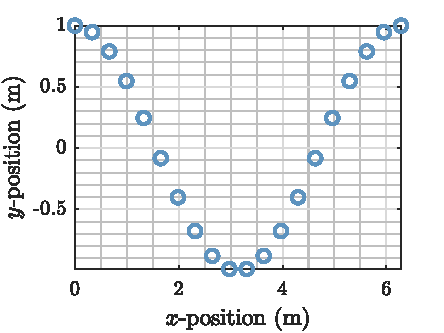
\includegraphics[width=\linewidth]{Images/Cos.pdf}
        \caption{Projectile 1}
        \label{fig:Projectile1}
    \end{subfigure}\hfill
    \begin{subfigure}[t]{0.49\columnwidth}
    \centering
        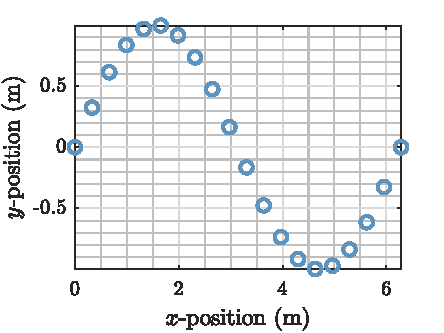
\includegraphics[width=\linewidth]{Images/Sin.pdf}
        \caption{Projectile 2}
        \label{fig:Projectile2}
    \end{subfigure}
    \caption{Trajectories of two projectiles as sub-figures.}
    \label{fig:Subfigs}
\end{figure}

Note that sometimes it is better to combine figures where datasets are being compared. In the case of the two projectiles shown in \Cref{fig:Projectile1} and \Cref{fig:Projectile2}, the data is easier to compare when shown as in \Cref{fig:OneFig}. When multiple datasets are shown on a single figure, remember:
\begin{itemize}
    \item Use different markers and colours to differentiate between the datasets. It is best practice to always use different markers. Reports may be shown in black and white and differentiating only by colour is not enough.
    \item Include a legend that does not obscure the data-points and has sufficiently descriptive names.
\end{itemize}
By combining the the datasets we can enlarge the figure width to enhance clarity while taking up the same amount of page space.

\begin{figure}
    \centering
    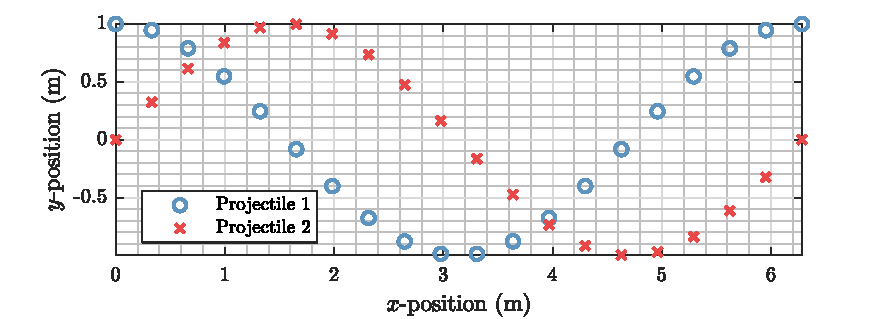
\includegraphics{Images/Both.pdf}
    \caption{Trajectories of two projectiles as a single figure.}
    \label{fig:OneFig}
\end{figure}

\section{Tables}
Tables are another good way to clearly format data. Table formatting rules vary between publications, though for university assignments there are some general rules to follow. As in \Cref{tab:Table}, some key points to remember when formatting tables are:
\begin{itemize}
    \item Table captions are always numbered and go \textbf{above} the table.
    \item As with figures, no table should be included unless it is directly referred to in your writing.
    \item Use appropriate significant figures when listing numbers.
    \item Always include units in the column header when the units for a given column are all the same.
    \item Reduce clutter by removing vertical separation lines and any double rules.
    \item Similarly, don't use colours if it isn't absolutely necessary.
    \item Group column headings where possible to clarify relationships between datasets.
\end{itemize}

\begin{table}
    \centering
    \caption{An example of a well formatted table.}
    \label{tab:Table}
    \begin{tabular}{@{}llr@{}} \toprule
    \multicolumn{2}{c}{Item} \\ \cmidrule(r){1-2}
    Animal & Description & Price (\$)\\ \midrule
    Gnat & per gram & 13.65 \\
    & each & 0.01 \\
    Gnu & stuffed & 92.50 \\
    Emu & stuffed & 33.33 \\
    Armadillo & frozen & 8.99 \\ \bottomrule
    \end{tabular}
\end{table}

\section{Referencing}
All work that isn't entirely your own must be referrenced. In some subjects you will be asked to refernce following a specific style guide. In this subject, we don't enforce a particular style, but you must remain consistent in your style. If you don't have a preferred referencing style, feel free to follow the \href{https://www.aiaa.org/publications/journals/reference-style-and-format}{AIAA Reference Style and Format Guide}. In engineering reports, footnote citation styles are generally avoided. Where a source is referenced in the text, it must be included in a bibliography at the end of the report. Bibliographies are generally not included in page counts. Below are some example citations so that you can see them in the bibliography:
\begin{itemize}
    \item \cite{dirac} is a book.
    \item \cite{einstein} is an article.
    \item \cite{knuthwebsite} is an online resource.
    \item \cite{knuth-fa} is a book chapter.
\end{itemize}

\clearpage
\backmatter{}
\printbibliography[heading=bibintoc]
% \listoftodos[Notes]
% Appendix ignored in word count
%%TC:ignore
% \clearpage
\begin{appendices}
\section{Appendix Example}
When writing reports, you may want to include information that is supplementary to the main body of the work. Generally appendices are not included in page counts. However, information in the appendix is also generally not assessed and you should assume markers will not look at the appendix when grading your work.
% 
\section{Style Guide Examples}\label{app:StyleGuide}
\subsection{General}
\begin{itemize}
    \item \href{https://www.ctan.org/tex-archive/info/l2tabu/english/}{l2tabu} is a comprehensive list of dos and don'ts and is considered ``required reading'' for \LaTeX{} users. More info can also be found \href{https://faculty.math.illinois.edu/~hildebr/tex/tips.html}{here} for general tips.
    \item Packages may become obsolete or conflict. \href{http://www.macfreek.nl/memory/LaTeX_package_conflicts}{LaTex Package Conflicts} is a good list of these.
    \item New lines can create unwanted space in the compiled document. To make more readable, use \% to comment blank lines before and after commands.
    \item Never break paragraphs using \verb|\\| or \verb|\par|. Add a blank line instead.
    \item Always make sure any compile errors and warnings have been resolved before completing a document.
\end{itemize}
% 
\subsection{Numbers \& Equations}
\begin{itemize}
    \item \LaTeX{} swallows spaces in math environments so add them where you see fit to make code more readable.
    \item The \verb|phyiscs| package defines many handy commands for typesetting equations in math environments. The full documentation can be found \href{https://ctan.org/pkg/physics?lang=en}{here}. Commonly used commands are in \Cref{tab:PhysicsCommands}.
    \begin{table*}
        \centering
        \caption{physics package commands}
        \label{tab:PhysicsCommands}
        \begin{tabular}{lll}
            \verb|\qty()| & $\verb|\qty(\dots)| \longrightarrow \qty(\dots)$ & automatic brace sizing \\
            \verb|\qty{}| & $\verb|\qty{\dots}| \longrightarrow \qty{\dots}$ & \\
            \verb|\qty[]| & $\verb|\qty[\dots]| \longrightarrow \qty[\dots]$ & \\
            \verb|\vectorbold| & $\verb|\vb{a}| \longrightarrow \vb{a}$ & bolded vectors \\
            \verb|\vectorarrow| & $\verb|\va{a}| \longrightarrow \va{a}$ & arrow bolded vectors \\
            \verb|\vectorunit| & $\verb|\vu{a}| \longrightarrow \vu{a}$ & unit bolded vectors \\
            \verb|\gradient| & $\verb|\grad{\Psi}| \longrightarrow \grad{\Psi}$ &  \\
            \verb|\divergence| & $\verb|\div{\Psi}| \longrightarrow \div{\Psi}$ &  \\
            \verb|\curl| & $\verb|\curl{\Psi}| \longrightarrow \curl{\Psi}$ &  \\
            \verb|\differential| & $\verb|\dd{x}|\ \longrightarrow \dd{x}$ & \\
            & $\verb|\dd[2]{x}|\ \longrightarrow \dd[2]{x}$ & \\
             \verb|\derivative| & $\verb|\dv{x}|\ \longrightarrow \dv{x}$ & \\
            & $\verb|\dv{y}{x}|\ \longrightarrow \dv{y}{x}$ & \\
            & $\verb|\dv[2]{y}{x}|\ \longrightarrow \dv[2]{y}{x}$ & \\
            \verb|\partialderivative| & $\verb|\pdv{x}|\ \longrightarrow \pdv{x}$ & \\
            & $\verb|\pdv{y}{x}|\ \longrightarrow \pdv{y}{x}$ & \\
            & $\verb|\pdv[2]{y}{x}|\ \longrightarrow \pdv[2]{y}{x}$ & \\
        \end{tabular}
    \end{table*}
    \begin{itemize}
        \item The standard set of trig functions is redefined in \verb|physics| to provide automatic braces that behave like \verb|\qty()| when used as \verb|\sin(...)|. 
    \end{itemize}
    \item The \verb|siunitx| package is useful for in-text numbers. Numbers should not be entered in text mode unless they are part of a name (e.g. Pixel 2XL). The full documentation can be found \href{https://ctan.org/pkg/siunitx?lang=en}{here}. Commonly used commands are in \Cref{tab:SiunitxCommands}.
    \begin{table*}
        \centering
        \caption{siunitx package commands}
        \label{tab:SiunitxCommands}
        \begin{tabular}{lll}
            \verb|\num{}| & $\verb|\num{123}| \longrightarrow \num{123}$ & consistent in-text numbers \\
            \verb|\ang{}| & $\verb|\ang{45}| \longrightarrow \ang{45}$ & proper degree symbol \\
            \verb|\si{}| & $\verb|\si{\m\per\s}| \longrightarrow \si{\m\per\s}$ & formatted SI units \\
            \verb|\si{}| & $\verb|\SI{123}{\m\per\s}| \longrightarrow \SI{123}{\m\per\s}$ & formatted SI units with number \\
        \end{tabular}
    \end{table*}
    \item Single line equation: \begin{equation}
    c^2 = a^2 + b^2
\end{equation}
    \item Aligned equations: \begin{align}
    \div{\vb{E}} &= \frac{\rho}{\varepsilon_0} \\
    \div{\vb{B}} &= 0 \\
    \curl{\vb{E}} &= -\pdv{\vb{B}}{t}\\
    \curl{\vb{B}} &= \mu_0\qty(\vb{J} + \varepsilon_0 \pdv{\vb{E}}{t})
\end{align}
    \item Sub-equations: \begin{subequations}
\begin{align}
    \oiint_{\partial\Omega} \vb{E} \vdot \dd{\vb{S}} &= \frac{1}{\varepsilon_0} \iiint_\Omega \rho \dd{V} \\
    \oiint_{\partial\Omega} \vb{B} \vdot \dd{\vb{S}} &= 0 \\
    \oint_{\partial \Sigma} \vb{E} \vdot \dd{\vb{l}} &= -\dv{t} \iint_\Sigma \vb{B} \vdot \dd{\vb{S}}
\end{align}
\end{subequations}
    \item Split equations: \begin{equation}
    \begin{split}
        y_1 + y_2 &= A\sin\qty(k x - \omega t) \\
        &+ A\sin\qty(k x + \omega t)
    \end{split}
\end{equation}
    \item Multiple equations in one line (avoid in general): \begin{multicols}{2}
    \noindent
    \begin{equation}
        C_L = \frac{L}{\frac{1}{2}\rho V^2 S}
    \end{equation}
    \begin{equation}
        C_D = \frac{D}{\frac{1}{2}\rho V^2 S}
    \end{equation}
\end{multicols}
\end{itemize}
% 
\subsection{Figures}
\begin{itemize}
    \item Standard figure: \Cref{fig:Standard}. Note that the \verb|width=\columnwidth| for figures placed in the body.
    \begin{figure}
    \centering
    \includegraphics[width=\columnwidth]{example-image-a}
    \caption{Caption}
    \label{fig:Standard}
\end{figure}
    \item Figure across two columns (specific to twocolumn option being used): \Cref{fig:TwoColumn}. Note that the \verb|width=\textwidth| for figures placed across all columns.
    \begin{figure*}
    \centering
    \includegraphics[width=\textwidth]{example-image-a}
    \caption{Caption}
    \label{fig:TwoColumn}
\end{figure*}
    \item Sub-figures: \Cref{fig:Subfigs}. Note that the third uncaptioned figure can be used for a legend or removed.
    \begin{figure}
    \centering
    \begin{subfigure}[t]{0.49\columnwidth}
    \centering
        \includegraphics[width=\linewidth]{example-image-a}
        \caption{Caption}
        \label{fig:SubfigA}
    \end{subfigure}\hfill
    \begin{subfigure}[t]{0.49\columnwidth}
    \centering
        \includegraphics[width=\linewidth]{example-image-b}
        \caption{Caption}
        \label{fig:SubfigB}
    \end{subfigure}
    % Remove below subfigure if separate legend is not necessary
    \vskip \abovecaptionskip 
    \begin{subfigure}[t]{0.49\columnwidth}
    \centering
        \includegraphics[width=\linewidth]{example-image-c}
    \end{subfigure}
    \caption{Caption}
    \label{fig:Subfigs}
\end{figure}
    \item Multiple figures in one line: \Cref{fig:Multifig1,fig:Multifig2}.
    \begin{figure}
    \centering
    \begin{minipage}[t]{0.49\columnwidth}
      \centering
        \includegraphics[width=\linewidth]{example-image-a}
        \caption{Caption}
        \label{fig:Multifig1}
    \end{minipage}\hfill
    \begin{minipage}[t]{0.49\columnwidth}
      \centering
        \includegraphics[width=\linewidth]{example-image-b}
        \caption{Caption}
        \label{fig:Multifig2}
    \end{minipage}%
\end{figure}
\end{itemize}
% 
\subsection{Tables}
\begin{itemize}
    \item Tables should generally adhere to formatting guidelines defined by the \href{https://ctan.org/pkg/booktabs?lang=en}{booktabs} package. The below templates are provided.
    \item For pages with more than one columns, the \verb|table*| environment can be used to span all columns.
    \item Standard table: \Cref{tab:Standard}. Note that \verb|\makecell[<anchor>]{<text\\text>}| can be used to split headers across multiple lines.
    \begin{table}
    \centering
    \caption{Caption}
    \label{tab:Standard}
    \begin{tabular}{lrr} \toprule
         Header 1 & Header 2 & \makecell[cr]{Header\\2} \\ \midrule
         Item 1 & 123456 & 789012 \\
         Item 2 & abcdef & ghijkl \\ \bottomrule
    \end{tabular}
\end{table}
    \item Subheadings with column rules: \Cref{tab:Subheadings}
    \begin{table}
    \centering
    \caption{Caption}
    \label{tab:Subheadings}
    \begin{tabular}{lrr} \toprule
        & \multicolumn{2}{c}{Header 2} \\ \cmidrule{2-3}
        Header 1 & Subheader 1 & Subheader 2 \\ \midrule
        Item 1 & 123456 & 789012 \\
        Item 2 & abcdef & ghijkl \\ \bottomrule
    \end{tabular}
\end{table}
    \item Set Width Table: \Cref{tab:SetWidth}
    \begin{table}
    \centering
    \caption{Caption}
    \label{tab:SetWidth}
    \begin{tabularx}{\columnwidth}{lrX} \toprule
         Header 1 & Header 2 & Header 3 \\ \midrule
         Item 1 & 123456 & This is a long paragraph that needs to be split over more than one line. This is another long paragraph that needs to be split over more than one line.\\
         Item 2 & abcdef &  This is a long paragraph that needs to be split over more than one line. This is another long paragraph that needs to be split over more than one line.\\ \bottomrule
    \end{tabularx}
\end{table}
    \item \verb|longtable| can also be used to create tables that break over more than one page.
\end{itemize}
% 
\subsection{Cross Referencing} 
\begin{itemize}
    \item Always use \verb|\{Cref{<label>}| for cross-referencing rather than \verb|Figure \ref{<label>}|, as the \verb|cleveref| package includes the label.
    \item Clickable URLs can be typeset with \verb|\href{<url>}{<text>}|, (e.g. \href{www.google.com}{Google}).
    \item References are typeset using \verb|biblatex| and can be printed using \verb|\printbibliography|. References are defined in \verb|refs.bib|, where templates are given for a number of document types.
\end{itemize}
% 
\subsection{Misc.}
\begin{itemize}
    \item ToDo items can be left with the \verb|\todo{<note>}| command and will render in the margin as well as in the Notes section if \verb|\listoftodos[Notes]| is present. \todo{This is what a TODO looks like.}
    \item Code can be typeset with the \verb|listings| package using \verb|\lstinputlisting{<path/to/code>}|. Currently syntax highlighting is set for MATLAB.
    \item Sections can be made landscape using the \verb|landscape| environment.
\end{itemize}
\end{appendices}
% 
%%TC:endignore
\end{document}
